\documentclass[8pt,aspectratio=169]{beamer}
\usetheme{Madrid}
\usepackage{graphicx}
\usepackage{booktabs}
\usepackage{adjustbox}
\usepackage{multicol}
\usepackage{amsmath}
\usepackage{listings}
\usepackage{xcolor}

% Color definitions
\definecolor{mlblue}{RGB}{0,102,204}
\definecolor{mlpurple}{RGB}{51,51,178}
\definecolor{mllavender}{RGB}{173,173,224}
\definecolor{mllavender2}{RGB}{193,193,232}
\definecolor{mllavender3}{RGB}{204,204,235}
\definecolor{mllavender4}{RGB}{214,214,239}
\definecolor{mlorange}{RGB}{255, 127, 14}
\definecolor{mlgreen}{RGB}{44, 160, 44}
\definecolor{mlred}{RGB}{214, 39, 40}
\definecolor{mlgray}{RGB}{127, 127, 127}

% Additional colors for template compatibility
\definecolor{lightgray}{RGB}{240, 240, 240}
\definecolor{midgray}{RGB}{180, 180, 180}

% Apply custom colors to Madrid theme
\setbeamercolor{palette primary}{bg=mllavender3,fg=mlpurple}
\setbeamercolor{palette secondary}{bg=mllavender2,fg=mlpurple}
\setbeamercolor{palette tertiary}{bg=mllavender,fg=white}
\setbeamercolor{palette quaternary}{bg=mlpurple,fg=white}

\setbeamercolor{structure}{fg=mlpurple}
\setbeamercolor{section in toc}{fg=mlpurple}
\setbeamercolor{subsection in toc}{fg=mlblue}
\setbeamercolor{title}{fg=mlpurple}
\setbeamercolor{frametitle}{fg=mlpurple,bg=mllavender3}
\setbeamercolor{block title}{bg=mllavender2,fg=mlpurple}
\setbeamercolor{block body}{bg=mllavender4,fg=black}

% Remove navigation symbols
\setbeamertemplate{navigation symbols}{}

% Clean itemize/enumerate
\setbeamertemplate{itemize items}[circle]
\setbeamertemplate{enumerate items}[default]

% Reduce margins for more content space
\setbeamersize{text margin left=5mm,text margin right=5mm}

% Command for bottom annotation (Madrid-style)
\newcommand{\bottomnote}[1]{%
\vfill
\vspace{-2mm}
\textcolor{mllavender2}{\rule{\textwidth}{0.4pt}}
\vspace{1mm}
\footnotesize
\textbf{#1}
}

% TikZ and pgfplots packages
\usepackage{tikz}
\usepackage{pgfplots}
\pgfplotsset{compat=1.18}
\usetikzlibrary{arrows.meta, positioning, shapes.geometric, calc, decorations.pathmorphing}

\title{Blockchain Fundamentals: Course Preview}
\subtitle{INTRO Preview -- What You Will Learn}
\author{Prof.~Dr.~Joerg Osterrieder}
\institute{University Lecture Series}
\date{\today}

\begin{document}

% ============================================================
% FRAME 1: Title slide
% ============================================================
\begin{frame}
  \titlepage
\end{frame}

% ============================================================
% FRAME 2: Block Anatomy (TikZ)
% ============================================================
\begin{frame}{Block Anatomy}
\begin{center}
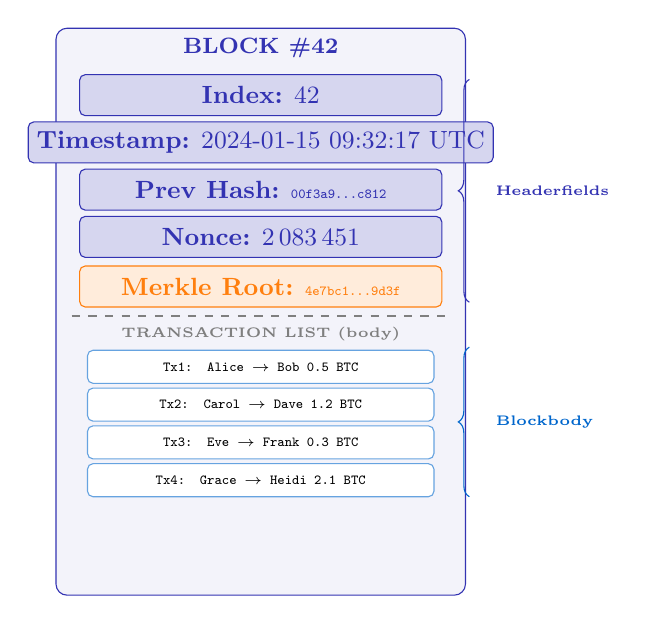
\begin{tikzpicture}[
    every node/.style={font=\small},
    field/.style={
        rectangle, rounded corners=2pt,
        minimum width=4.6cm, minimum height=0.52cm,
        text centered, inner sep=3pt
    },
    header/.style={field, draw=mlpurple, fill=mllavender4, text=mlpurple},
    body/.style={field, draw=mlblue, fill=mllavender3!60, text=mlblue},
    tx/.style={field, draw=mlblue!60, fill=white, text=black,
               minimum width=4.4cm, minimum height=0.42cm},
    label/.style={font=\tiny\bfseries, text=mlgray},
    brace/.style={decorate, decoration={brace, mirror, amplitude=4pt}},
]

% ---- Block outer rectangle ----
\node[draw=mlpurple, fill=mllavender4!30, rounded corners=4pt,
      minimum width=5.2cm, minimum height=7.2cm] (block) at (0,0) {};

% ---- "BLOCK #42" label ----
\node[font=\footnotesize\bfseries, text=mlpurple] at (0, 3.35) {BLOCK \#42};

% ---- Header fields ----
\node[header] (idx)  at (0,  2.75) {\textbf{Index:} 42};
\node[header] (ts)   at (0,  2.15) {\textbf{Timestamp:} 2024-01-15 09:32:17 UTC};
\node[header] (prev) at (0,  1.55) {\textbf{Prev Hash:} \texttt{\tiny 00f3a9...c812}};
\node[header] (non)  at (0,  0.95) {\textbf{Nonce:} 2\,083\,451};

% ---- Merkle root (orange accent) ----
\node[field, draw=mlorange, fill=mlorange!15, text=mlorange] (mr) at (0, 0.32)
      {\textbf{Merkle Root:} \texttt{\tiny 4e7bc1...9d3f}};

% ---- Divider ----
\draw[mlgray, dashed, thick] (-2.4,-0.05) -- (2.4,-0.05);

% ---- Transaction list label ----
\node[label] at (0,-0.28) {TRANSACTION LIST (body)};

% ---- Transactions ----
\node[tx] (t1) at (0,-0.70) {\texttt{\tiny Tx1: Alice $\to$ Bob  0.5 BTC}};
\node[tx] (t2) at (0,-1.18) {\texttt{\tiny Tx2: Carol $\to$ Dave  1.2 BTC}};
\node[tx] (t3) at (0,-1.66) {\texttt{\tiny Tx3: Eve   $\to$ Frank 0.3 BTC}};
\node[tx] (t4) at (0,-2.14) {\texttt{\tiny Tx4: Grace $\to$ Heidi 2.1 BTC}};

% ---- Side labels ----
\draw[brace, mlpurple] (2.65, 2.95) -- (2.65, 0.12)
      node[midway, right=6pt, label, text=mlpurple] {Header\\fields};
\draw[brace, mlblue]  (2.65,-0.45) -- (2.65,-2.35)
      node[midway, right=6pt, label, text=mlblue]  {Block\\body};

\end{tikzpicture}
\end{center}
\bottomnote{Each block bundles a set of transactions under a tamper-evident header linked to its predecessor.}
\end{frame}

% ============================================================
% FRAME 3: Hash Linking and Merkle Trees (TikZ)
% ============================================================
\begin{frame}{Hash Linking and Merkle Trees}
\begin{center}
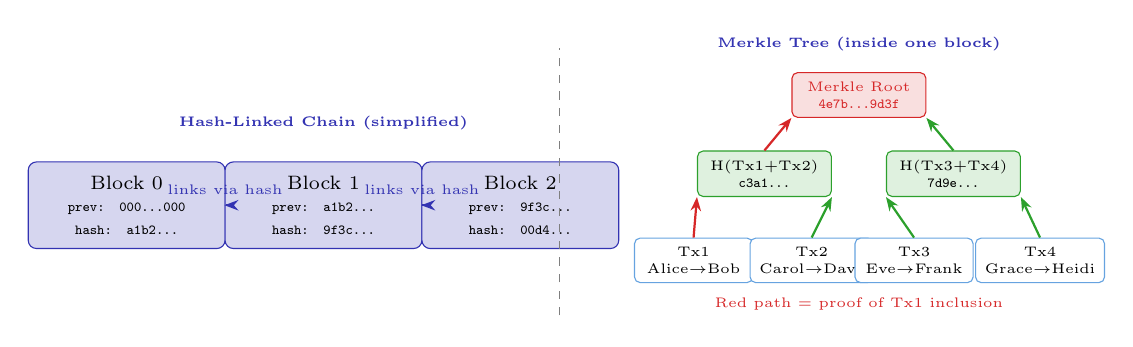
\begin{tikzpicture}[
    every node/.style={font=\scriptsize},
    blk/.style={draw=mlpurple, fill=mllavender4, rounded corners=3pt,
                minimum width=2.5cm, minimum height=1.1cm, align=center},
    hashnode/.style={draw=mlgreen, fill=mlgreen!15, rounded corners=2pt,
                     minimum width=1.7cm, minimum height=0.45cm, align=center,
                     font=\tiny},
    txnode/.style={draw=mlblue!60, fill=white, rounded corners=2pt,
                   minimum width=1.5cm, minimum height=0.4cm,
                   font=\tiny, align=center},
    arr/.style={-{Stealth[length=5pt]}, thick},
    redarr/.style={-{Stealth[length=5pt]}, thick, mlred},
]

% ===== LEFT SIDE: chain of three blocks =====
\node[blk] (B0) at (-5.5, 0.8) {Block 0\\{\tiny \texttt{prev: 000...000}}\\{\tiny \texttt{hash: a1b2...}}};
\node[blk] (B1) at (-3.0, 0.8) {Block 1\\{\tiny \texttt{prev: a1b2...}}\\{\tiny \texttt{hash: 9f3c...}}};
\node[blk] (B2) at (-0.5, 0.8) {Block 2\\{\tiny \texttt{prev: 9f3c...}}\\{\tiny \texttt{hash: 00d4...}}};

% hash arrows
\draw[arr, mlpurple] (B0.east) -- (B1.west)
      node[midway, above, font=\tiny, text=mlpurple] {links via hash};
\draw[arr, mlpurple] (B1.east) -- (B2.west)
      node[midway, above, font=\tiny, text=mlpurple] {links via hash};

% label
\node[font=\tiny\bfseries, text=mlpurple] at (-3.0, 1.85) {Hash-Linked Chain (simplified)};

% ===== RIGHT SIDE: Merkle tree (inside Block 2 body) =====
% Root
\node[hashnode, draw=mlred, fill=mlred!15, text=mlred] (root) at (3.8, 2.2)
      {Merkle Root\\{\tiny \texttt{4e7b...9d3f}}};

% Level 1
\node[hashnode] (h01) at (2.6, 1.2) {H(Tx1+Tx2)\\{\tiny \texttt{c3a1...}}};
\node[hashnode] (h23) at (5.0, 1.2) {H(Tx3+Tx4)\\{\tiny \texttt{7d9e...}}};

% Level 2 (leaves)
\node[txnode] (tx1) at (1.7, 0.1)  {Tx1\\{\tiny Alice$\to$Bob}};
\node[txnode] (tx2) at (3.2, 0.1)  {Tx2\\{\tiny Carol$\to$Dave}};
\node[txnode] (tx3) at (4.5, 0.1)  {Tx3\\{\tiny Eve$\to$Frank}};
\node[txnode] (tx4) at (6.1, 0.1)  {Tx4\\{\tiny Grace$\to$Heidi}};

% tree edges (red path to highlight Tx1 verification)
\draw[redarr] (tx1.north) -- (h01.south west);
\draw[arr, mlgreen] (tx2.north) -- (h01.south east);
\draw[arr, mlgreen] (tx3.north) -- (h23.south west);
\draw[arr, mlgreen] (tx4.north) -- (h23.south east);
\draw[redarr] (h01.north) -- (root.south west);
\draw[arr, mlgreen] (h23.north) -- (root.south east);

% labels
\node[font=\tiny\bfseries, text=mlpurple] at (3.8, 2.85)
      {Merkle Tree (inside one block)};
\node[font=\tiny, text=mlred]   at (3.8,-0.45)
      {Red path = proof of Tx1 inclusion};

% vertical separator
\draw[mlgray, dashed] (-0.0, -0.6) -- (-0.0, 2.8);

\end{tikzpicture}
\end{center}
\bottomnote{Hash chaining ensures tamper-evidence; Merkle trees enable lightweight transaction proof without downloading the full block.}
\end{frame}

% ============================================================
% FRAME 4: PoW vs PoS Energy Consumption (pgfplots bar chart)
% ============================================================
\begin{frame}{Proof-of-Work vs.\ Proof-of-Stake: Energy Footprint}
\begin{center}
\begin{tikzpicture}
\begin{axis}[
    ybar,
    bar width=22pt,
    width=0.82\textwidth,
    height=0.72\textheight,
    ylabel={Energy Consumption (TWh / year)},
    ylabel style={font=\small},
    symbolic x coords={Bitcoin (PoW), Eth pre-merge (PoW), Ethereum (PoS), Cardano (PoS)},
    xtick=data,
    x tick label style={font=\small, align=center, text width=2.8cm},
    ymin=0, ymax=175,
    ytick={0,25,50,75,100,125,150,175},
    yticklabel style={font=\small},
    nodes near coords,
    nodes near coords style={font=\scriptsize\bfseries, /pgf/number format/fixed,
                             /pgf/number format/precision=2},
    enlarge x limits=0.18,
    grid=major,
    grid style={draw=mlgray!30, dashed},
    axis line style={mlgray},
    tick style={mlgray},
    legend pos=north east,
    legend style={font=\small, draw=mlgray!50},
]
% PoW bars (red)
\addplot[fill=mlred!80, draw=mlred!60] coordinates {
    (Bitcoin (PoW),         150)
    (Eth pre-merge (PoW),    78)
};
% PoS bars (green) -- rendered separately so we can split by color
\addplot[fill=mlgreen!75, draw=mlgreen!60] coordinates {
    (Ethereum (PoS),        0.01)
    (Cardano (PoS),         0.006)
};
\legend{Proof-of-Work, Proof-of-Stake}
\end{axis}
\end{tikzpicture}
\end{center}
\bottomnote{Switching consensus from PoW to PoS reduced Ethereum's energy use by $\approx$99.95\,\% -- a key sustainability milestone for the industry.}
\end{frame}

% ============================================================
% FRAME 5: Decentralization Spectrum (pgfplots scatter)
% ============================================================
\begin{frame}{Decentralization Spectrum of Major Blockchain Projects}
\begin{center}
\begin{tikzpicture}
\begin{axis}[
    width=0.9\textwidth,
    height=0.68\textheight,
    xmin=-0.5, xmax=10.5,
    ymin=0,    ymax=6,
    xlabel={Decentralization Score (0 = fully centralized, 10 = fully decentralized)},
    xlabel style={font=\small},
    ytick=\empty,
    xtick={0,1,2,3,4,5,6,7,8,9,10},
    xticklabel style={font=\small},
    grid=major,
    grid style={draw=mlgray!25, dashed},
    axis line style={mlgray},
    tick style={mlgray},
    clip=false,
]

% Spectrum gradient bar at y=0.5
\addplot[fill=mllavender3, draw=none, ybar interval, opacity=0.4]
    coordinates {(0,0.1)(10,0.1)} \closedcycle;

% Background arrow annotation
\draw[-{Stealth[length=8pt]}, mlgray, thick] (axis cs:0,0.3) -- (axis cs:10,0.3)
      node[right, font=\tiny, text=mlgray] {more decentralized};

% Project points
% Visa (centralized) -- mlred
\addplot[only marks, mark=*, mark size=5pt, mlred]
    coordinates {(1, 2)};
\node[font=\small\bfseries, text=mlred, above] at (axis cs:1,2.1) {Visa};
\node[font=\tiny, text=mlgray, below] at (axis cs:1,1.85) {score 1};

% Ripple -- mlorange
\addplot[only marks, mark=*, mark size=5pt, mlorange]
    coordinates {(3, 3)};
\node[font=\small\bfseries, text=mlorange, above] at (axis cs:3,3.1) {Ripple (XRP)};
\node[font=\tiny, text=mlgray, below] at (axis cs:3,2.85) {score 3};

% BSC -- mlgray
\addplot[only marks, mark=*, mark size=5pt, mlgray]
    coordinates {(4, 2)};
\node[font=\small\bfseries, text=mlgray, above] at (axis cs:4,2.1) {Binance SC};
\node[font=\tiny, text=mlgray, below] at (axis cs:4,1.85) {score 4};

% Ethereum -- mlblue
\addplot[only marks, mark=*, mark size=5pt, mlblue]
    coordinates {(7, 4)};
\node[font=\small\bfseries, text=mlblue, above] at (axis cs:7,4.1) {Ethereum};
\node[font=\tiny, text=mlgray, below] at (axis cs:7,3.85) {score 7};

% Bitcoin -- mlgreen
\addplot[only marks, mark=*, mark size=5pt, mlgreen]
    coordinates {(9, 3)};
\node[font=\small\bfseries, text=mlgreen, above] at (axis cs:9,3.1) {Bitcoin};
\node[font=\tiny, text=mlgray, below] at (axis cs:9,2.85) {score 9};

% Labels at extremes
\node[font=\tiny\bfseries, text=mlred,   align=center] at (axis cs:0,5.3) {Fully\\Centralized};
\node[font=\tiny\bfseries, text=mlgreen, align=center] at (axis cs:10,5.3) {Fully\\Decentralized};

\end{axis}
\end{tikzpicture}
\end{center}
\bottomnote{Decentralization is a spectrum, not a binary property -- projects trade control for scalability, speed, and governance flexibility.}
\end{frame}

% ============================================================
% FRAME 6: Blockchain Adoption Trends (pgfplots line chart)
% ============================================================
\begin{frame}{Blockchain Adoption Trends: Wallet Growth}
\begin{center}
\begin{tikzpicture}
\begin{axis}[
    width=0.88\textwidth,
    height=0.72\textheight,
    xlabel={Year},
    ylabel={Blockchain Wallets (millions)},
    xlabel style={font=\small},
    ylabel style={font=\small},
    xmin=2014.5, xmax=2023.5,
    ymin=0, ymax=105,
    xtick={2015,2016,2017,2018,2019,2020,2021,2022,2023},
    xticklabel style={font=\small},
    ytick={0,10,20,30,40,50,60,70,80,90,100},
    yticklabel style={font=\small},
    grid=major,
    grid style={draw=mlgray!25, dashed},
    axis line style={mlgray},
    tick style={mlgray},
    legend pos=north west,
    legend style={font=\small, draw=mlgray!50},
]

% Shaded area under curve
\addplot[fill=mlblue!12, draw=none] coordinates {
    (2015,  5)
    (2016, 10)
    (2017, 22)
    (2018, 32)
    (2019, 44)
    (2020, 62)
    (2021, 80)
    (2022, 85)
    (2023, 90)
    (2023,  0)
    (2015,  0)
} \closedcycle;

% Main line
\addplot[
    color=mlblue,
    thick,
    mark=*,
    mark options={fill=mlblue, draw=mlpurple, line width=0.6pt},
    mark size=3.5pt,
] coordinates {
    (2015,  5)
    (2016, 10)
    (2017, 22)
    (2018, 32)
    (2019, 44)
    (2020, 62)
    (2021, 80)
    (2022, 85)
    (2023, 90)
};
\addlegendentry{Global blockchain wallets}

% Annotate the 2017 surge
\draw[mlred, dashed, -{Stealth[length=5pt]}]
      (axis cs:2017.3, 35) -- (axis cs:2017, 23)
      node[above right, font=\tiny, text=mlred, at start] {2017 crypto boom};

% Annotate 2021 peak growth
\draw[mlgreen, dashed, -{Stealth[length=5pt]}]
      (axis cs:2021.3, 68) -- (axis cs:2021, 81)
      node[below right, font=\tiny, text=mlgreen, at start] {DeFi \& NFT surge};

% Data labels on key points
\node[font=\tiny\bfseries, text=mlblue, above left]  at (axis cs:2015, 5)  {5M};
\node[font=\tiny\bfseries, text=mlblue, above]        at (axis cs:2017, 22) {22M};
\node[font=\tiny\bfseries, text=mlblue, above left]   at (axis cs:2020, 62) {62M};
\node[font=\tiny\bfseries, text=mlblue, above right]  at (axis cs:2023, 90) {90M};

\end{axis}
\end{tikzpicture}
\end{center}
\bottomnote{Global blockchain wallet count grew $\approx$18$\times$ between 2015 and 2023, reflecting accelerating mainstream and institutional adoption.}
\end{frame}

\end{document}
